\subsection{Sufficient Geometric Conditions for Continuous Global Coverage}
\label{subsec:geometric_conditions}

Для обеспечения непрерывного глобального покрытия поверхности Земли орбитальной 
группировкой типа Уокера необходимо выполнение набора взаимодополняющих геометрических 
ограничений. Эти ограничения возникают вследствие специфики взаимного расположения 
орбитальных плоскостей и определяют характер перекрытия полос покрытия в различных
узлах сферической геометрии. В рамках сферической модели Земли, поскольку реальный 
эллипсоид вписан в сферу, удовлетворение нижеприведённых неравенств является 
достаточным для обеспечения непрерывности покрытия и для реальной земной поверхности.

Выделение трёх отдельных аспектов — коорбитального, ретроградного и полярного — 
обусловлено исчерпывающим охватом всех возможных взаимных конфигураций плоскостей
в группировке Уокера. С точки зрения теории спутниковых орбит, эти три условия 
соответствуют трём типам относительного движения соседних плоскостей: движению 
в одном направлении, движению в противоположных направлениях и сходящемуся 
движению в высоких широтах. Их совместное выполнение формирует полную систему
достаточных условий, исключающую разрывы покрытия как в экваториально-средних, 
так и в приполярных регионах.

To achieve global coverage, three groups of geometric conditions must be satisfied, accounting for
the mutual arrangement of the orbital planes. These include co-orbital, retrograde, and polar
conditions. It is important to note that these conditions are sufficient for the spherical Earth
model. Since the Earth's ellipsoid is inscribed within this sphere,
satisfying these inequalities guarantees full coverage for the actual ellipsoidal model as well.

% ToDo define coordital, retrograde and polar condition and explain how it works
Let adjacent orbital planes be called co-orbital if the spacecraft in them move in the same
direction. To prevent coverage gaps between these planes, the distance between them must not exceed
the maximum allowable value \(D\). Geometrically, this distance is defined as the sum of half the
coverage strip of one plane and the field-of-view radius of the adjacent one:

\begin{equation}
    D = \lambda_{\text{street}} + \theta.
\end{equation}

Adjacent planes in which spacecraft move in opposite directions are called retrograde. In a Walker
constellation, these are the first and last planes.

For retrograde planes, the maximum allowable angular distance between them is defined as the sum of
two coverage strips:
\begin{equation}
    D_{re} = 2\lambda_{\text{street}}.
\end{equation}

In polar case we have a ''claw'', which appears when the inclination of orbits less then $$90^{\circ}$$.


Задачу обеспечения непрерывного глобального покрытия можно разложить на 
три независимые геометрические подзадачи, которые зависят от расположения 
орбитальных плоскостей (рисунок~\ref{fig:geometric_conditions_overview}). 
Мы выделяем три критически важные конфигурации, которые должны быть удовлетворены 
для гарантии глобального покрытия: коорбитальные, ретроградные и полярные условия. 
Необходимость рассматривать эти аспекты по отдельности обусловлена различным 
движением спутников относительно друг друга.

Коорбитальные плоскости показаны на рисунке~\ref{fig:coorbital_condition} (а). 
В рамках группировки Уокера фазовый сдвиг между космическими аппаратами в соседних 
плоскостях является фиксированным параметром, а аппараты в пределах одной плоскости 
разнесены на равные интервалы по аргументу широты. Следовательно, для обеспечения 
непрерывности перекрытия полос покрытия максимально допустимое угловое расстояние 
между плоскостями ограничено величиной
\begin{equation}
D = \lambda_{\text{street}} + \theta,
\end{equation}

Ретроградная конфигурация проиллюстрирована на рисунке~\ref{fig:retrograde_condition} (б). 
В этом случае относительное движение аппаратов в соседних плоскостях происходит навстречу 
друг другу. Следовательно, суммарная угловая протяженность группировки не должна превышать значение
\begin{equation}
D_{re} = 2\lambda_{\text{street}}.
\end{equation}

В полярной области, из-за того что наклонение орбит меньше $$90^{\circ}$$, у полюса 
образуется незакрытая область в форме «когтя» (см. рисунок~\ref{fig:polar_condition}, в). 
Закрыть её можно только за счёт ширины полос покрытия, которые должны доставать до самой оси вращения.

Совместное выполнение всех трех условий обеспечивает отсутствие разрывов 
покрытия во всех широтных зонах.

The problem of ensuring continuous global coverage can be decomposed 
into three independent geometric sub-problems that depend on the arrangement 
of the orbital planes (Figure~\ref{fig:geometric_conditions_overview}).
We identify three critical configurations that must be satisfied to 
guarantee global coverage: co-orbital, retrograde, and polar conditions. 
The need to consider these aspects separately is driven by the different 
relative motion of the satellites. 

Co-orbital planes are shown in Figure~\ref{fig:coorbital_condition} (a). 
Within the Walker constellation framework, the phase shift between spacecraft 
in adjacent planes is a fixed parameter, and spacecraft within a single plane 
are separated by equal intervals in argument of latitude. Consequently, 
to ensure continuous overlap of the coverage strips, the maximum allowable 
angular distance between the planes is limited by 
\begin{equation}
    D = \lambda_{\text{street}} + \theta,
\end{equation}

The retrograde configuration is illustrated in Figure~\ref{fig:retrograde_condition} (b). 
In this case, the relative motion of spacecraft in adjacent planes occurs towards each other. 
Consequently, the total angular extent of the constellation must not exceed 
\begin{equation}
    D_{re} = 2\lambda_{\text{street}}.
\end{equation}

In the polar region, because the orbital inclination is less than \(90^\circ\), an 
uncovered "claw-shaped" region forms near the pole (see Figure~\ref{fig:polar_condition}, c). 
It can only be closed by the width of the coverage strips, which must extend all the way to 
the axis of rotation.

The joint fulfillment of all three conditions ensures the absence of coverage gaps in 
all latitudinal zones.

\begin{figure}[ht]
    \centering
    \begin{subfigure}[b]{0.32\textwidth}
        \centering
        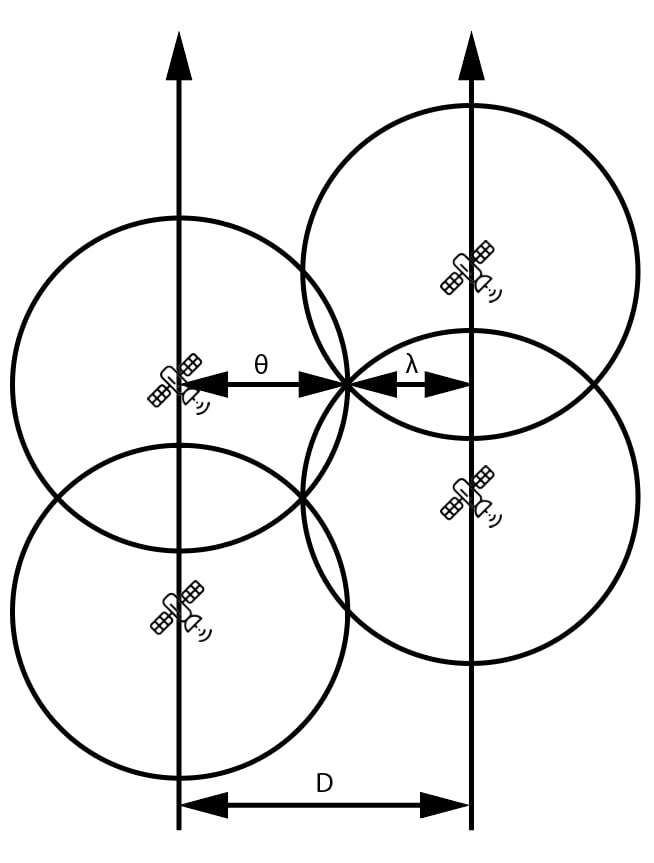
\includegraphics[width=\linewidth]{pictures/coorbital_condition.jpg}
        \caption{Коорбитальные плоскости: соседние плоскости движутся в одном направлении; показаны полоса покрытия и фазовый сдвиг.}
        \label{fig:coorbital_condition}
    \end{subfigure}\hfill
    \begin{subfigure}[b]{0.32\textwidth}
        \centering
        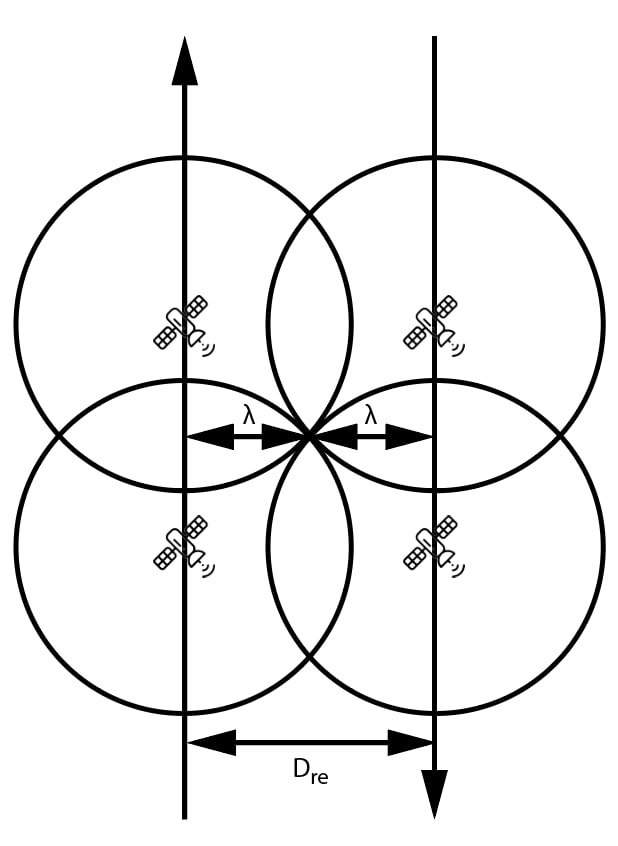
\includegraphics[width=\linewidth]{pictures/retrograde_condition.jpg}
        \caption{Ретроградные условия: соседние плоскости движутся в противоположных направлениях; показан суммарный эффект полос покрытия.}
        \label{fig:retrograde_condition}
    \end{subfigure}\hfill
    \begin{subfigure}[b]{0.32\textwidth}
        \centering
        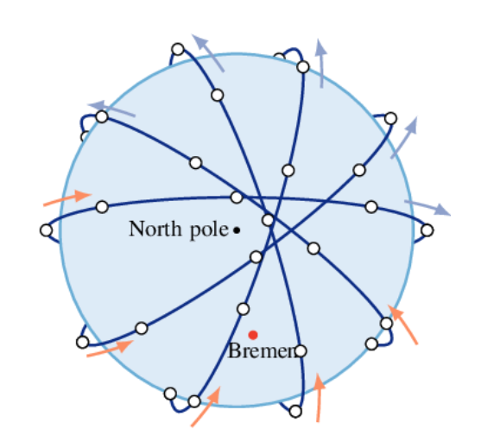
\includegraphics[width=\linewidth]{pictures/polar_condition.png}
        \caption{Полярные условия: иллюстрация области вокруг полюса и требование перекрытия "claw"-области для обеспечения покрытия.}
        \label{fig:polar_condition}
    \end{subfigure}
    \caption{Ознакомительные схемы геометрических условий покрытия: (а) коорбитальные, (б) ретроградные, (в) полярные.}
    \label{fig:geometric_conditions_overview}
\end{figure}

\paragraph{Conditions for Co-Orbital Planes}

% Let adjacent orbital planes be called co-orbital if the spacecraft in them move in the same
% direction. To prevent coverage gaps between these planes, the distance between them must not exceed
% the maximum allowable value \(D\). Geometrically, this distance is defined as the sum of half the
% coverage strip of one plane and the field-of-view radius of the adjacent one:
% \begin{equation}
%     D = \lambda_{\text{street}} + \theta.
% \end{equation}

Based on the normal vectors to the orbital planes, the angular distance between two co-orbital
planes \(i_{rel}\) is expressed through the inclination and the RAAN difference as:
\begin{equation}
    \cos i_{rel} = \cos^2 i + \cos(\Delta\Omega) \sin^2 i.
\end{equation}

Equating this distance to the maximum allowable value (\(i_{rel} = D\)), we obtain the restriction
on the maximum RAAN difference for co-orbital planes:
\begin{equation}\label{eq:delta_omega_max}
    \Delta\Omega_{\text{max}} = \arccos\left(\frac{\cos D - \cos^2 i}{\sin^2 i}\right).
\end{equation}
Choosing \(\Delta\Omega \leq \Delta\Omega_{\text{max}}\) ensures that no gaps in coorbital planes.

\begin{figure}[ht]
    \centering
    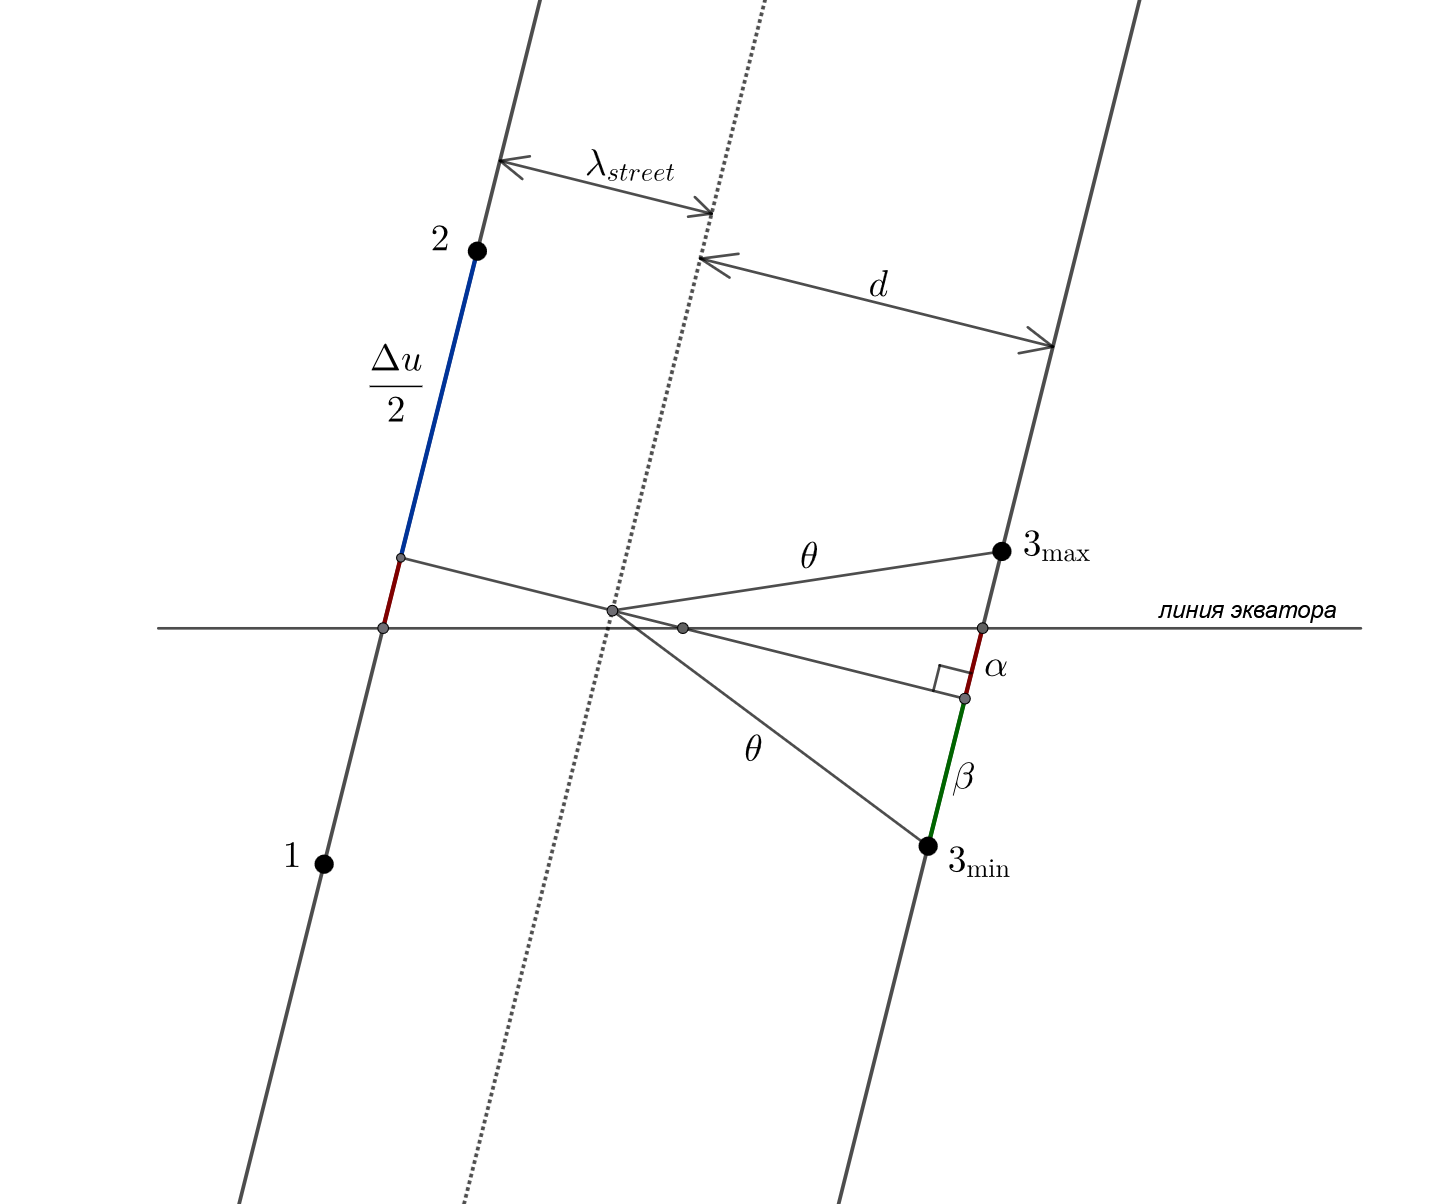
\includegraphics[width=0.75\textwidth]{pictures/phase_shift.png}
    \caption{Diagram of the phase shift between adjacent orbital planes}
    \label{fig:phase_shift}
\end{figure}

Furthermore, for co-orbital planes, the influence of the phase shift \(f\) must be considered. This
shift determines the relative offset of the ground tracks along the intersection of two adjacent
planes and, consequently, how the coverage strips overlap. Figure~\ref{fig:phase_shift} illustrates
the mutual geometry of the orbits with a phase shift. We consider two adjacent co-orbital planes
with a RAAN difference of $\Delta\Omega$. We assume that the chosen $\Delta\Omega$ lies within the
allowable RAAN range. The angular distance between these planes is denoted as $i_{rel}$.

Since the coverage strip of a single orbit has a width of $\lambda_{\text{street}}$, the angular
distance from the outer edge of one orbit's coverage strip to the adjacent orbit along the arc
$i_{rel}$ is:
\begin{equation}
    d = i_{rel} - \lambda_{\text{street}}.
\end{equation}

To avoid a coverage gap, the spacecraft on the adjacent orbit must be positioned sufficiently close
to the boundary of the first orbit's coverage strip. Geometrically, this implies that the angular
distance between the spacecraft on the adjacent orbit and the strip boundary must not exceed the
central field-of-view angle $\theta$.

On the left orbit, the first spacecraft is located \(\Delta u/2\) downward from the intersection of
the arc \(i_{rel}\), while the second spacecraft is located \(\Delta u/2\) upward. Let us denote the
allowable range of the argument of latitude for the spacecraft on the adjacent orbit as
\(u_{3,\min}\) and \(u_{3,\max}\).

We measure the phase shift from the first spacecraft on the left orbit upwards along the direction
of motion. If \(u_3\) falls within the range \([u_{3,\min}, u_{3,\max}]\), no coverage gaps will
occur between the adjacent planes. The allowable phase shifts are then expressed as:
\begin{equation}\label{eq:phase_shift}
    f_{max} = \frac{\Delta u}{2} + \beta - 2\alpha
\end{equation}
\begin{equation}
    f_{min} = \frac{\Delta u}{2} - \beta - 2\alpha
\end{equation}

From spherical geometry, we can express the allowable deviation in argument of latitude $\beta$ and
the offset $\alpha$:
\begin{equation}
    \beta = \arccos \left(  \frac{\cos \theta}{\cos d} \right)
\end{equation}
\begin{equation}
    \alpha = \arccos \left( \frac{\cos(\frac{\Delta\Omega}{2})}{\cos(\frac{i_{rel}}{2})} \right)
\end{equation}

By substituting the expressions for \(\alpha\) and \(\beta\) into \eqref{eq:phase_shift}, we obtain
the final analytical formulas for calculating the phase shift boundaries:
\begin{equation}
    f_{max} = \frac{\Delta u}{2} + \arccos \left( \frac{\cos \theta}{\cos d} \right)
    - 2 \arccos \left( \frac{\cos\left(\frac{\Delta\Omega}{2}\right)}{\cos\left(
        \frac{i_{rel}}{2}\right)} \right)
\end{equation}
\begin{equation}
    f_{min} = \frac{\Delta u}{2} - \arccos \left( \frac{\cos \theta}{\cos d} \right)
    - 2 \arccos \left( \frac{\cos\left(\frac{\Delta\Omega}{2}\right)}{\cos\left(
        \frac{i_{rel}}{2}\right)} \right)
\end{equation}

Selecting a phase shift \(f \in [f_{\min}, f_{\max}]\) guarantees continuous coverage between
co-orbital planes.


\paragraph{Conditions for Retrograde Planes}

% Adjacent planes in which spacecraft move in opposite directions are called retrograde. In a Walker
% constellation, these are the first and last planes.

For a given number of planes \(P\), the longitude of the ascending node of the last plane is
determined as:
\begin{equation}
    \Omega_P = (P-1)\Delta\Omega_{\text{max}},
\end{equation}
where \(\Delta\Omega_{\text{max}}\) is the maximum RAAN step obtained for the co-orbital planes
(\ref{eq:delta_omega_max}).

If \(\Delta\Omega_{\text{max}} < \pi\), it is necessary to verify whether a coverage gap exists on
the retrograde orbits.

% For retrograde planes, the maximum allowable angular distance between them is defined as the sum of
% two coverage strips:
% \begin{equation}
%     D_{re} = 2\lambda_{\text{street}}.
% \end{equation}

The angular distance between the first and last planes can be computed as follows:
\begin{equation}
    \cos i_{rel} = \cos^2 i + \cos\bigl((P-1)\Delta\Omega_{\text{max}}\bigr)\sin^2 i.
\end{equation}
This distance \(i_{rel}\) corresponds to the angle between the planes when measured between their
ascending nodes.

To assess the coverage gap between retrograde planes, we must determine the angle measured
specifically between these retrograde planes. It is given by:
\begin{equation}
    i_{rel}^{(re)} = \pi - i_{rel}.
\end{equation}
If the condition \(i_{rel}^{(re)} \leq D_{re}\) holds, the coverage on the retrograde planes remains
continuous. Otherwise, a coverage gap occurs.

Unlike the co-orbital case, the phase shift \(f\) has no effect on the coverage on retrograde
orbits. The planes move toward each other, and their mutual geometric position remains fixed at any
given moment.

Equating the angular distance between the first and last planes \(i_{rel}^{(re)}\) to \(D_{re}\), we
obtain the expression for the minimum allowable RAAN difference at which no coverage gap occurs:
\begin{equation}
    \Delta\Omega_{\text{min}} = \frac{1}{(P-1)} \arccos\left(
        \frac{-\cos D_{re} - \cos^2 i}{\sin^2 i}\right).
\end{equation}

Thus, for retrograde planes, the RAAN difference is chosen based on the condition \(\Delta\Omega
\geq \Delta\Omega_{\text{min}}\). In this case, the geometric position of such planes remains fixed
during satellite motion, and the phase shift does not influence the continuity of coverage.

\paragraph{Polar Conditions}

Earth pole coverage requires specific analysis. For orbits with inclinations less than $90^\circ$, 
the projections of satellite trajectories onto the Earth's surface do not pass through the poles. 
Instead, the ground tracks reach their maximum latitude corresponding to the orbital inclination. 
Even if the Walker constellation parameters are chosen such that no coverage gaps occur between adjacent 
orbital planes, a ''claw'' shaped region around the pole may remain uncovered (Fig.~~\ref{fig:polar_claw}).
\begin{figure}[ht]
    \centering
    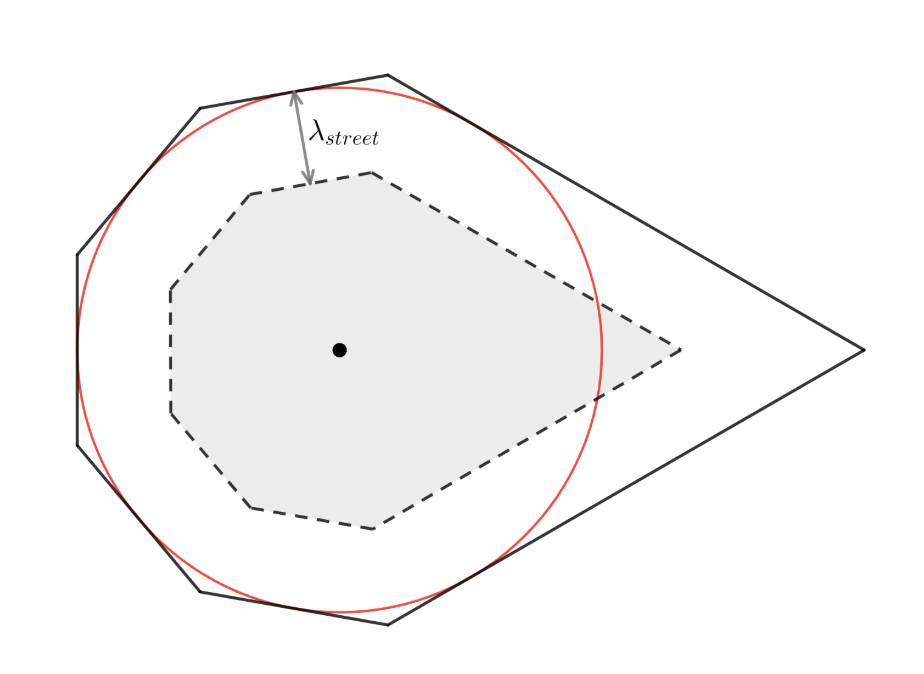
\includegraphics[width=0.75\textwidth]{pictures/polar_claw.png}
    \caption{Uncovered polar polygon: red circle - points with latitude corresponding to the orbital inclination}
    \label{fig:polar_claw}
\end{figure}
If all groundtrack projections near the pole are expanded by the street-of-coverage half-width 
$\lambda_{\mathrm{street}}$, the remaining region forms the polygon of interest. 
To ensure that this region remains covered, the following condition must be satisfied:

\begin{equation}
    \lambda_{\mathrm{street}} \geq \left|\frac{\pi}{2}-i\right|.
\end{equation}

Under this condition, the streets-of-coverage of all orbital planes pass through the pole in 
the worst-case configuration and cover the otherwise uncovered region. This constraint is imposed on 
the streets of coverage to account for retrograde orbits.
The traditional condition \(\lambda_{\mathrm{street}} > 0\) \cite{wertz2001ocdm} is achieved only in the limited case of \(i=\frac{\pi}{2}\).
    
    
